\documentclass[letterpaper, 12pt]{article}
\usepackage[top=2 cm, bottom=2 cm,left=1.5 cm, right=1.5 cm]{geometry}

\usepackage[spanish,es-nodecimaldot]{babel}
\usepackage[utf8]{inputenc}
\usepackage{csquotes}

\setlength{\parindent}{1cm}
\pagestyle{empty}

\usepackage{amsmath}
\usepackage[outputdir=aux]{minted}
\usepackage{amssymb}
\usepackage{multicol}
\usepackage{enumerate}
\usepackage{graphicx} % Incluir imágenes
\usepackage[document]{ragged2e}
\usepackage{mathrsfs}
\usepackage[T1]{fontenc}
\usepackage[table,xcdraw]{xcolor}
\usepackage{float} %required for the placement specifier H
\makeatletter
\makeatother
% -----------------------------------------------

% Preámbulo

\title{Tarea 2: }
\author{Christopher Gómez}
\date{Marzo 2022}

\begin{document}
\parbox[t]{.5\linewidth}{
    \centering
    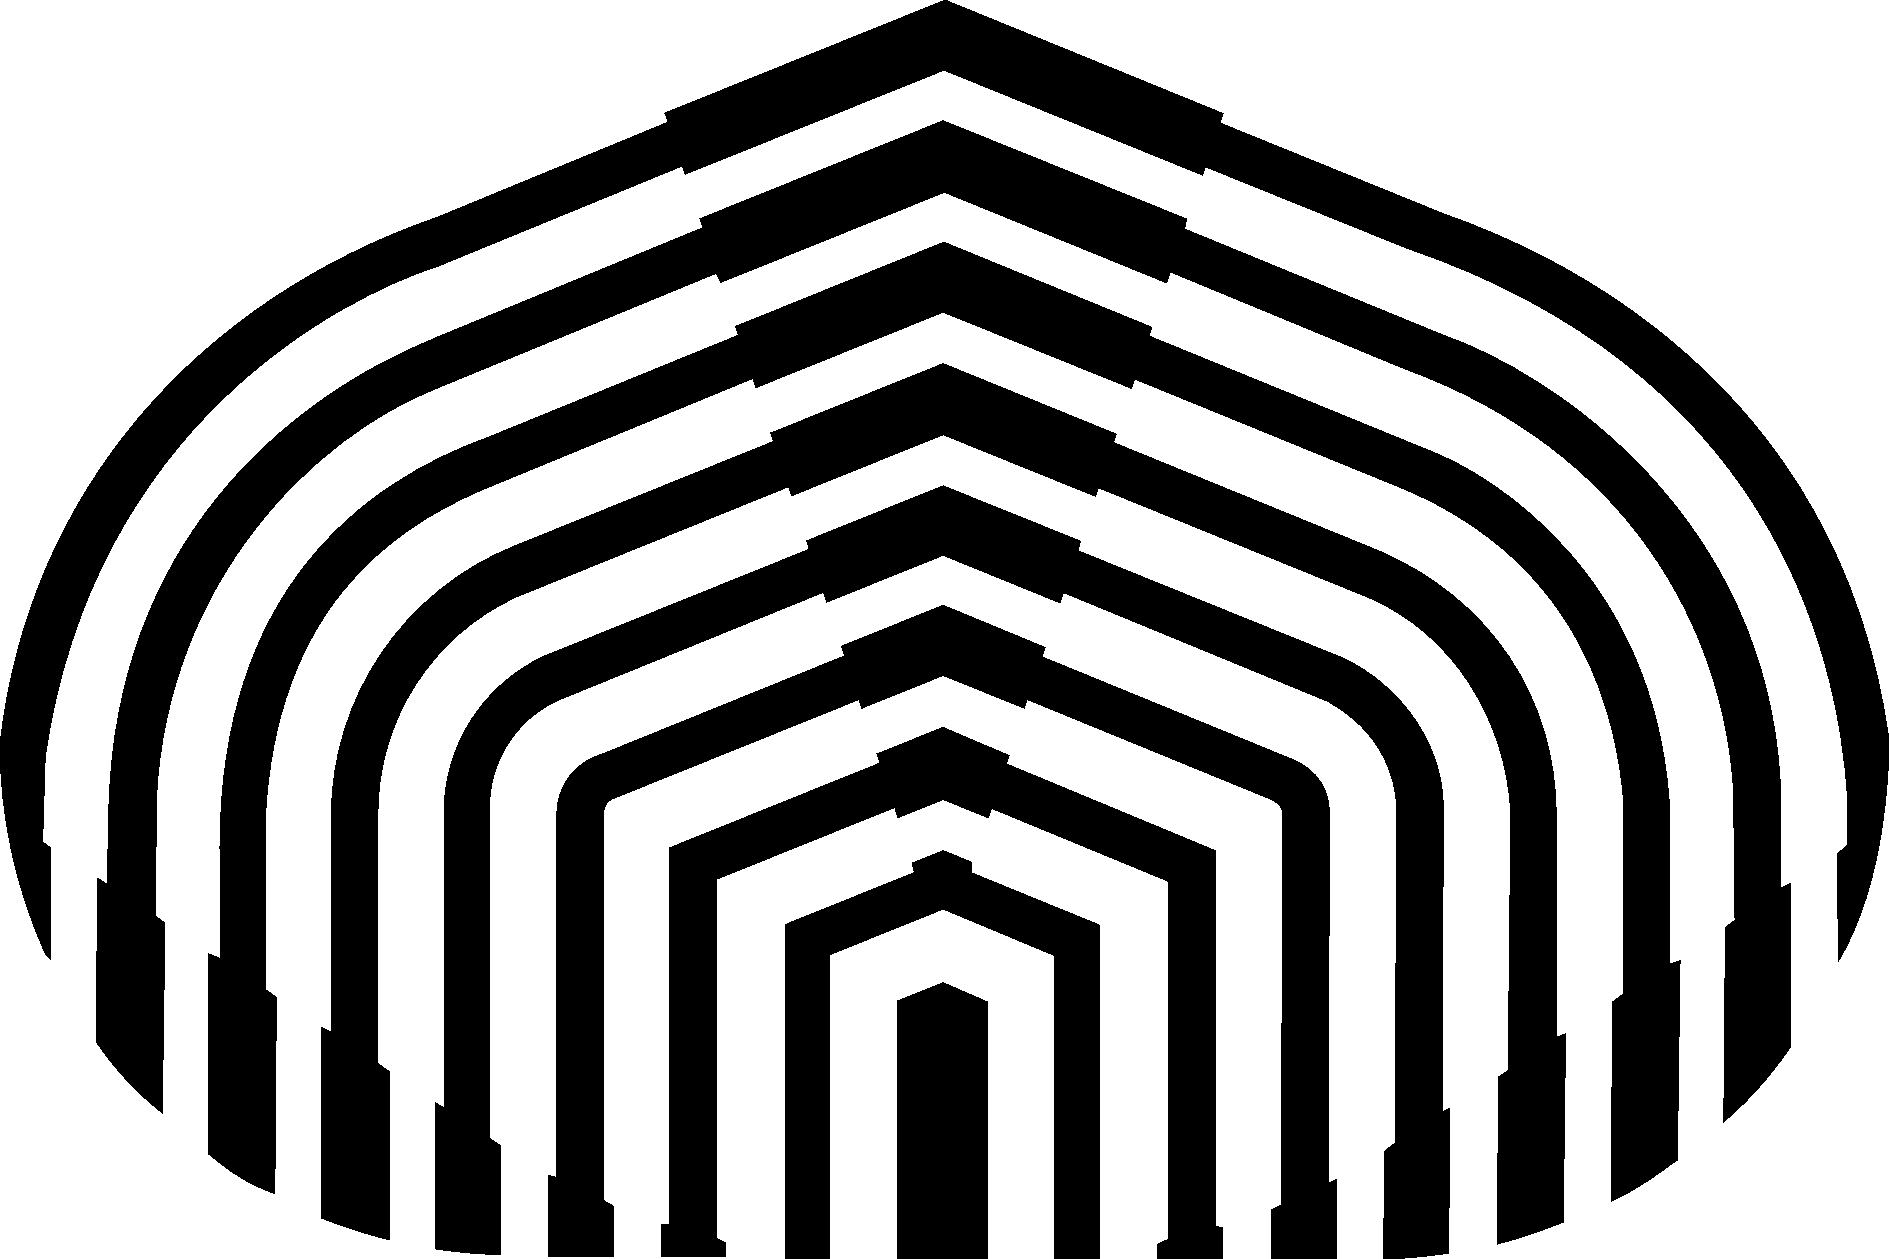
\includegraphics[scale=0.4]{logo.png}
    \begin{center}
        UNIVERSIDAD SIMÓN BOLÍVAR \\
        CI-5651 - Diseño de Algoritmos I \\
        Prof. Ricardo Monascal \\
    \end{center}
}
\hfill \framebox[5.5cm][c]{
        \parbox[t]{.8\linewidth}{
        \centering
       Resuelto por:\\ Christopher Gómez
        }}

\phantom{This text will be invisible} \\
\centerline {\textbf{Tarea 2: }}
\justify

\begin{enumerate}

% -------- PREGUNTA 1 --------

\item  En un nuevo túnel, diversos productos quieren colocar vallas para promover
sus productos. Usted debe dar los permisos apropiados para colocar estas vallas y no desea que ninguna de estas se intersecte con otra (sin embargo, dos vallas pueden estar una al lado de la otra, esto es, compartir un extremo).

Las propuestas de publicidad incluyen el punto en donde la valla empezará (en metros, contando desde el inicio del túnel) y el tamaño de la misma (también en metros). Ninguna de estas condiciones es negociable. Los departamentos de publicidad de cada uno de los productos interesados han llegado a la conclusión de que quieren la valla en ese exacto punto, con esas exactas dimensiones o prefieren no colocar publicidad alguna. Todas las vallas se colocarán planas en una sola pared del túnel.

Dadas $n$ peticiones de publicidad, donde la $i$-ésima petición tiene $p_i$ (el punto de inicio de la valla) y $t_i$ (el tamaño de la valla), diseñe un algoritmo \emph{eficiente} que permite escoger un conjunto maximal de peticiones tal que ninguna valla intersecte con otra.

Por ejemplo, considere que $n = 3$ y las peticiones son:

\begin{itemize}
    \item $p_1 = 1$ y $t_1 = 4$
    \item $p_2 = 2$ y $t_2 = 1$
    \item $p_3 = 3$ y $t_3 = 3$
\end{itemize}

Un conjunto maximal sería $\{2, 3\}$, cubriendo los rangos $[2..3]$ y $[3..6]$.

Su algoritmo debe usar tiempo $O(n\log n)$ y memoria adicional $O(n)$.

Justifique \emph{informalmente} por qué su algoritmos es correcto y cumple con el orden asintótico propuesto.

Además del informe expresando su solución, debe dar una implementación de su solución en el lenguaje de su elección (solamente como una función; el formato de entrada/salida no es relevante).


% -------- PREGUNTA 2 --------


\item Considere las siguientes definiciones:

\textbf{Conjuntos definitivos de firmas funcionales}

Considere un conjunto de tipos $T$ y sea $F$ todas las firmas de funciones posibles entre los tipos de $T$ .

Por ejemplo, si $T = \{A, B, C\}$ entonces $F$ contiene

\begin{multicols}{3}
\begin{itemize}
    \item $A \rightarrow A$
    \item $A \rightarrow B$
    \item $A \rightarrow C$
    \item $B \rightarrow A$
    \item $B \rightarrow B$
    \item $B \rightarrow C$
    \item $C \rightarrow A$
    \item $C \rightarrow B$
    \item $C \rightarrow C$
\end{itemize}
\end{multicols}

Diremos que un subconjunto $F' \subseteq F$ es \emph{definitivo} si cada tipo ocurrente en $F'$ aparece a lo sumo una vez como imagen en $F'$.

Por ejemplo, para el mismo $T$ anterior:

\begin{itemize}
    \item $\{A \rightarrow B, B \rightarrow C\}$ es definitivo
    \item $\{A \rightarrow B, C \rightarrow B\}$ no es definitivo.
\end{itemize}

\textbf{Matroide asociada}

Dado un conjunto de tipos $T$ y su conjunto de todas las firmas de funciones $F$, definimos $M_T = (F, I)$, donde $F' \in I$ si y sólo si $F'$ es definitivo. \\

\textbf{Potencial de una firma funcional}

Definimos el \emph{potencial} de una firma de función $X \rightarrow Y$ como la cantidad de funciones posibles que existen con $X$ como dominio y $Y$ como imagen. Recordemos que esto es igual a $|Y|^{|X|}$. Puede suponer que todos los tipos tienen al menos un elemento ($T$ no contiene al tipo vacío).

El potencial de un conjunto de firmas de funciones es la suma del potencial para cada una de la firmas que contiene.

Se desea que:

a) Demuestre que $M_T$ es una matroide.
b) Plantee una función de costo $w$ de tal forma que para la matroide pesada $M_T$ , con $w$ como función de peso, los sub-conjuntos óptimos son los subconjuntos \emph{definitivos} con \emph{potencial máximo}.

\end{enumerate} \vspace{4mm}

\end{document}


|   |   |   |   |
  1   2   3
